\documentclass[a4paper, 11pt]{article}
\usepackage[text={17cm, 24cm}, left=2cm, top=3cm]{geometry}
\usepackage{times}
\usepackage[czech]{babel}
\usepackage[utf8]{inputenc}
\usepackage[hidelinks, unicode]{hyperref}
\usepackage{multirow}
\usepackage[czech, linesnumbered, longend, noline, ruled]{algorithm2e}
\usepackage{graphics}
\usepackage{lscape}

\begin{document}
\begin{titlepage}
    \begin{center}
       \textsc {\Huge{Vysoké učení technické v~Brně}\\
                \huge{Fakulta informačních technologií}\\}
        \vspace{\stretch{0.382}}
        {\LARGE Typografie a~publikování\,--\,3. projekt\\}
        {\Huge Tabulky a~obrázky}
        \vspace{\stretch{0.618}}
    \end{center}
    {\Large \today \hfill Simona Jánošíková}
\end{titlepage}

\section{Úvodní strana}
Název práce umístěte do zlatého řezu a~nezapomeňte uvést \uv{dnešní} (today) datum a~vaše jméno a~příjmení.

\section{Tabulky}
Pro sázení tabulek můžeme použít buď prostředí\verb| tabbing |nebo prostředí\verb| tabular|.

\subsection{Prostředí \texttt{tabbing}}
Při použití\verb| tabbing |vypadá tabulka následovně:

\begin{tabbing}
    Vodní melouny \quad	 \= \textbf{Cena} \quad	 \= \textbf{Množství} \kill
    \textbf{Ovoce}       \> \textbf{Cena}        \> \textbf{Množství}\\
    Jablka               \> 25,90                \> 3 kg\\
    Hrušky               \> 27,40                \> 2,5 kg\\
    Vodní melouny        \> 35,--                \> 1 kus
\end{tabbing}
Toto prostředí se dá také použít pro sázení algoritmů, ovšem vhodnější je použít prostředí\texttt{ algorithm }nebo\texttt{ algorithm2e }(viz sekce~\ref{sekcia3Algoritmy}).

\subsection{Prostředí \texttt{tabular}}
Další možností, jak vytvořit tabulku, je použít prostředí \verb|tabular|. Tabulky pak budou vypadat takto\footnote{Kdyby byl problem s\texttt{ cline, }zkuste se podívat třeba sem: \href{http://www.abclinuxu.cz/tex/poradna/show/325037}{http://www.abclinuxu.cz/tex/poradna/show/325037}.}:

\bigskip

\begin{table}[h]
    \centering
    \catcode`-=12
    \begin{tabular}{|l|c|c|}
        \hline
                        &\multicolumn{2}{c|}{\textbf{Cena}}\\ \cline{2-3} 
        \textbf{Měna}   &\textbf{nákup} &\textbf{prodej}\\ \hline
        EUR             &22,705         &25,242\\
        GBP             &25,931         &28,828\\
        USD             &21,347         &23,732\\ \hline
    \end{tabular}
    \caption{Tabulka kurzů k~dnešnímu dni}\label{tabulka_kurzy}
\end{table}

\bigskip

\begin{table}[h]
    \centering
    \catcode`-=12
    \begin{tabular}{|c|c|}
    \hline
	$A$	       & ${\neg}A$\\ \hline
	\textbf{P} & N\\ \hline
	\textbf{O} & O\\ \hline
	\textbf{X} & X\\ \hline
	\textbf{N} & P\\ \hline
    \end{tabular}
    \begin{tabular}{|c|c|c|c|c|c|}
    \hline
    \multicolumn{2}{|c}{\multirow{2}{*}{$A \wedge B$}} & \multicolumn{4}{|c|}{$B$}\\ \cline{3-6}
    \multicolumn{2}{|c|}{} & \textbf{P} & \textbf{O} & \textbf{X} & \textbf{N}\\ \hline
    \multirow{4}{*}{$A$} & \textbf{P} & P & O & X & N\\ \cline{2-6}
                         & \textbf{O} & O & O & N & N\\ \cline{2-6}
                         & \textbf{X} & X & N & X & N\\ \cline{2-6}
                         & \textbf{N} & N & N & N & N\\ \cline{2-6} \hline 
    \end{tabular}
    \begin{tabular}{|c|c|c|c|c|c|}
    \hline
    \multicolumn{2}{|c}{\multirow{2}{*}{$A \vee B$}} & \multicolumn{4}{|c|}{$B$}\\ \cline{3-6}
    \multicolumn{2}{|c|}{} & \textbf{P} & \textbf{O} & \textbf{X} & \textbf{N}\\ \hline
    \multirow{4}{*}{$A$} & \textbf{P} & P & P & P & P\\ \cline{2-6}
                         & \textbf{O} & P & O & P & O\\ \cline{2-6}
                         & \textbf{X} & P & P & X & X\\ \cline{2-6}
                         & \textbf{N} & P & O & X & N\\ \cline{2-6} \hline 
    \end{tabular}
    \begin{tabular}{|c|c|c|c|c|c|}
    \hline
    \multicolumn{2}{|c}{\multirow{2}{*}{$A \rightarrow B$}} & \multicolumn{4}{|c|}{$B$}\\ \cline{3-6}
    \multicolumn{2}{|c|}{} & \textbf{P} & \textbf{O} & \textbf{X} & \textbf{N}\\ \hline
    \multirow{4}{*}{$A$} & \textbf{P} & P & O & X & N\\ \cline{2-6}
                         & \textbf{O} & P & O & P & O\\ \cline{2-6}
                         & \textbf{X} & P & P & X & X\\ \cline{2-6}
                         & \textbf{N} & P & P & P & P\\ \cline{2-6} \hline 
    \end{tabular}
    \caption{Protože Kleeneho trojhodnotová logika už je \uv{zastaralá}, uvádíme si zde příklad čtyřhodnotové logiky}
    \label{tabulka_logika}
\end{table}

\bigskip
\pagebreak

\section{Algoritmy}\label{sekcia3Algoritmy}
Pokud budeme chtít vysázet algoritmus, můžeme použít prostředí\verb| algorithm|\footnote{Pro nápovědu, jak zacházet s~prostředím\texttt{ algorithm, }můžeme zkusit tuhle stránku:\\ \href{http://ftp.cstug.cz/pub/tex/CTAN/macros/latex/contrib/algorithms/algorithms.pdf}{http://ftp.cstug.cz/pub/tex/CTAN/macros/latex/contrib/algorithms/algorithms.pdf}.}  
nebo\verb| algorithm2e|\footnote{Pro \texttt{algorithm2e} zase tuhle: \href{http://ftp.cstug.cz/pub/tex/CTAN/macros/latex/contrib/algorithm2e/doc/algorithm2e.pdf}{http://ftp.cstug.cz/pub/tex/CTAN/macros/latex/contrib/algorithm2e/doc/algorithm2e.pdf}.}. Příklad použití prostředí \verb|algorithm2e| viz Algoritmus~\ref{algoritmus}.

\begin{algorithm}\label{algoritmus}
    \caption{\textsc{FastSLAM}}
    \KwIn{$(X_{t-1}, u_t, z_t)$}
    \KwOut{$X_t$}
    \SetNlSty{}{}{:}
    \BlankLine
    \SetNlSkip{-0.4cm}
    \Indp \Indp
    $\overline{X_{t}}=X_{t}=0$\\
    \For{$k = 1 \textrm{\emph{ to }} M$}{
        $x_t^{[k]} = \emph{sample\_motion\_model}(u_t, x_{t - 1}^{[k]})$\\
        $\omega_t^{[k]} = \emph{measurement\_model}(z_t, x_t^{[k]}, m_{t - 1})$\\
        $m_t^{[k]} = updated\_occupancy\_grid(z_t, x_t^{[k]}, m_{t - 1}^{[k]})$\\
        $\overline{X_t} = \overline{X_t} + \langle x_x^{[m]}, \omega_t^{[m]} \rangle$\\
    }
    \For{$k = 1 \textrm{\emph{ to }} M$}{
        draw $i$ with probability $\approx \omega_t^{[i]}$\\
        add $\langle x_x^{[k]}, m_t^{[k]} \rangle \textrm{ to } X_t$\\
    }
    \KwRet{$X_t$}
\end{algorithm}

\section{Obrázky}
Do našich článků můžeme samozřejmě vkládat obrázky. Pokud je obrázkem fotografie, můžeme klidně použít bitmapový soubor. Pokud by to ale mělo být nějaké schéma nebo něco podobného, je dobrým zvykem takovýto obrázek vytvořit vektorově.

\begin{figure}[h]
    \begin{center}
        \scalebox{0.4}{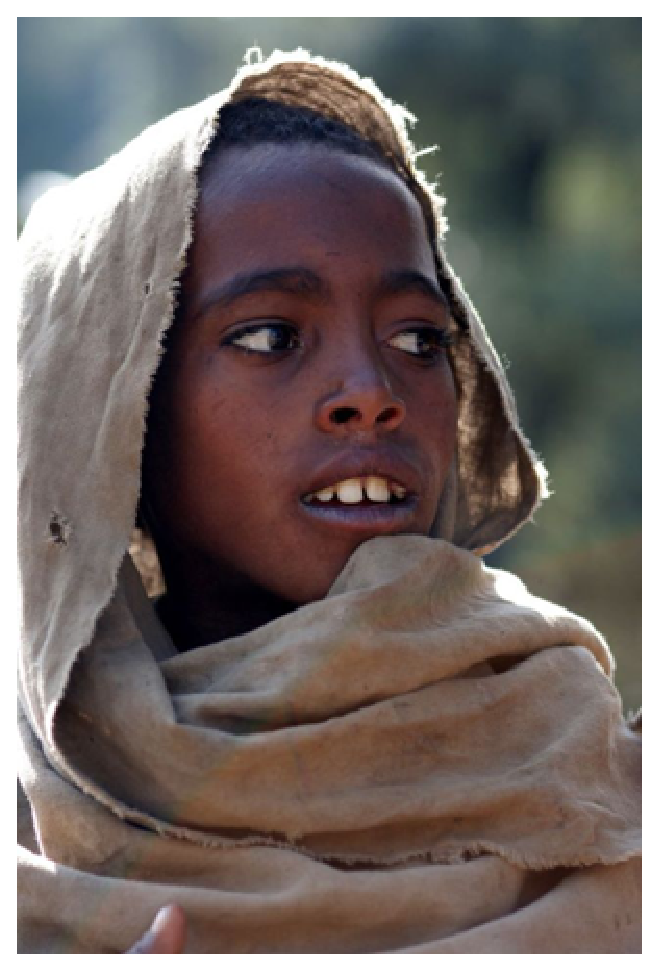
\includegraphics{etiopan.eps} \reflectbox{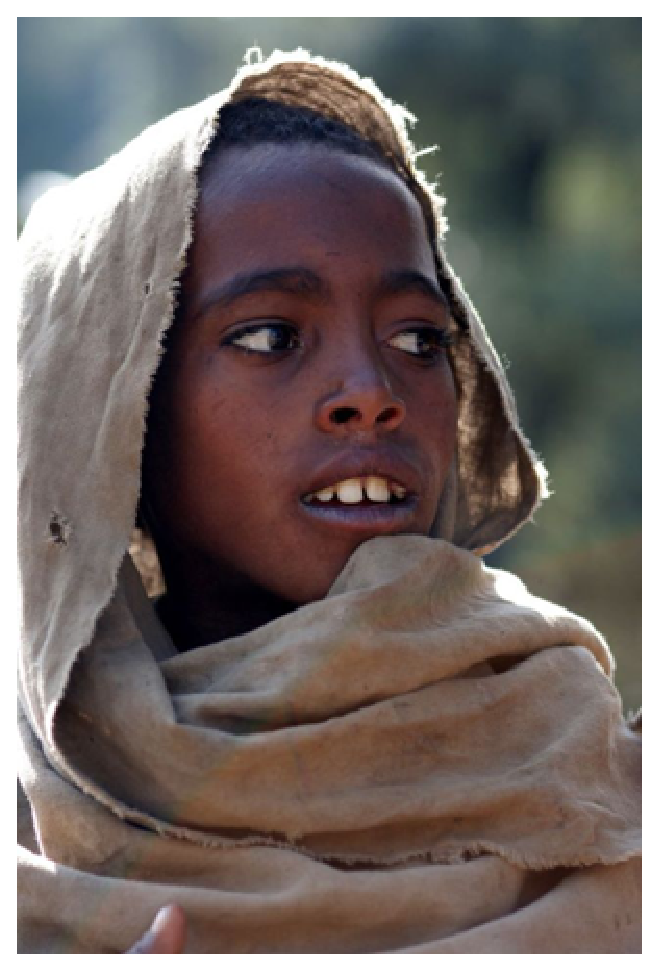
\includegraphics{etiopan.eps}}}
    \caption{Malý Etiopánek a~jeho bratříček}\label{OBR1}
    \end{center}
\end{figure}

Rozdíl mezi vektorovým \dots\\
\begin{figure}[h]
    \begin{center}
        \scalebox{0.4}{
\includegraphics{oniisan.eps}}
        \caption{Vektorový obrázek}\label{OBR2}
    \end{center}
\end{figure}
\\ \noindent \dots  a~bitmapovým obrázkem\\
\begin{figure}[h]
    \begin{center}
        \scalebox{0.6}{
\includegraphics{oniisan2.eps}}
        \caption{Bitmapový obrázek}\label{OBR3}
    \end{center}
\end{figure}
\\ \noindent se projeví například při zvětšení.


Odkazy (nejen ty) na obrázky~\ref{OBR1},~\ref{OBR2} a~\ref{OBR3}, na tabulky~\ref{tabulka_kurzy} a~\ref{tabulka_logika} a~také na algoritmus~\ref{algoritmus} jsou udělány pomocí křížových odkazů. Pak je ovšem potřeba zdrojový soubor přeložit dvakrát.

Vektorové obrázky lze vytvořit i~přímo v~\LaTeX u, například pomocí prostředí\verb| picture|.

\newpage

\begin{landscape}
    \begin{figure}[h]
        \setlength{\unitlength}{1mm}
        \centering
        \begin{picture}(200, 108)
            \linethickness{1pt}
            \put(0, 0){\framebox(200, 100){}}
            \linethickness{1pt}

            \put(25, 85){\circle{10}}

            %obrys
            \put(65, 32){\line(0, 0){60}}
            \put(60, 92){\line(1, 0){140}}
            \put(60, 92){\line(2, 1){16}}
            \put(65, 32){\line(1, 1){10}}
            \put(75, 42){\line(1, 0){55}}
            \put(134, 42){\line(1, 0){16}}
            \put(150, 42){\line(-1, -1){42}}
            \put(150, 8){\line(0, 0){34}}
            \put(150, 8){\line(-1, -1){8}}
            \put(150, 8){\line(1, 0){50}}
            
            %vchod
            \put(50, 50){\line(0, 0){20}}
            \put(50, 50){\line(1, 0){15}}
            \put(45, 70){\line(1, 0){20}}
            \put(45, 70){\line(2, 1){10}}
            \put(55, 75){\line(1, 0){10}}
            \put(55, 50){\line(0, 0){15}}
            \put(63, 50){\line(0, 0){15}}
            \put(55, 65){\line(1, 0){8}}
            \put(60, 57){\line(1, 0){2}}
            
            %plot + schody
            \put(0, 29){\line(2, 1){50}}
            \put(0, 43){\line(2, 1){50}}
            \put(40, 45){\line(2, 1){10}}
            \put(40, 45){\line(1, 0){25}}
            \put(40, 41){\line(0, 0){4}}
            \put(40, 41){\line(1, 0){25}}
            \put(36, 39){\line(2, 1){4}}
            \put(20, 39){\line(1, 0){45}}
            \put(20, 36){\line(0, 0){3}}
            \put(20, 36){\line(1, 0){45}}
            \put(16, 34){\line(2, 1){4}}
            \put(16, 34){\line(1, 0){49}}
            \put(16, 32){\line(1, 0){49}}
            \put(16, 32){\line(0, 0){2}}
            \put(0, 24){\line(2, 1){16}}
            \put(5, 0){\line(0, 0){20}}
            \put(0, 20){\line(1, 0){5}}
            \put(9, 4){\line(0, 0){20}}
            \put(5, 20){\line(1, 1){4}}
            \put(0, 20){\line(1, 1){4}}
            \put(4, 24){\line(1, 0){5}}
            \put(5, 0){\line(1, 1){4}}
            \put(88, 0){\line(0, 0){20}}
            \put(83, 0){\line(0, 0){20}}
            \put(83, 20){\line(1, 0){5}}
            \put(92, 4){\line(0, 0){20}}
            \put(88, 20){\line(1, 1){4}}
            \put(83, 20){\line(1, 1){4}}
            \put(87, 24){\line(1, 0){5}}
            \put(88, 0){\line(1, 1){4}}
            \put(108, 0){\line(0, 0){20}}
            \put(103, 0){\line(0, 0){20}}
            \put(103, 20){\line(1, 0){5}}
            \put(112, 4){\line(0, 0){20}}
            \put(108, 20){\line(1, 1){4}}
            \put(103, 20){\line(1, 1){4}}
            \put(107, 24){\line(1, 0){5}}
            \put(130, 22){\line(0, 0){20}}
            \put(125, 22){\line(0, 0){20}}
            \put(125, 22){\line(1, 0){5}}
            \put(134, 26){\line(0, 0){20}}
            \put(130, 42){\line(1, 1){4}}
            \put(125, 42){\line(1, 1){4}}
            \put(129, 46){\line(1, 0){5}}
            \put(112, 8){\line(1, 1){16}}
            \put(112, 18){\line(1, 1){16}}
            \put(134, 40){\line(1, 1){12}}
            \put(134, 30){\line(1, 1){12}}
            \put(146, 40){\vector(0, 0){15}}
            \put(141, 35){\vector(0, 0){15}}
            \put(136, 30){\vector(0, 0){15}}
            \put(124, 18){\vector(0, 0){15}}
            \put(120, 14){\vector(0, 0){15}}
            \put(115, 9){\vector(0, 0){15}}
            \put(90, 5){\line(1, 0){13}}
            \put(90, 17){\line(1, 0){13}}
            \put(90, 12){\line(1, 0){5}}
            \put(90, 5){\line(0, 0){12}}
            \put(93, 3){\vector(0, 0){17}}
            \put(97, 3){\vector(0, 0){17}}
            \put(101, 3){\vector(0, 0){17}}
            \put(7, 17){\line(1, 0){37}}
            \put(45, 17){\line(1, 0){38}}
            \put(7, 5){\line(1, 0){37}}
            \put(45, 5){\line(1, 0){38}}
            \put(44, 5){\line(0, 0){12}}
            \put(45, 5){\line(0, 0){12}}
            \put(10, 3){\vector(0, 0){17}}
            \put(15, 3){\vector(0, 0){17}}
            \put(20, 3){\vector(0, 0){17}}
            \put(25, 3){\vector(0, 0){17}}
            \put(30, 3){\vector(0, 0){17}}
            \put(35, 3){\vector(0, 0){17}}
            \put(40, 3){\vector(0, 0){17}}
            \put(50, 3){\vector(0, 0){17}}
            \put(55, 3){\vector(0, 0){17}}
            \put(60, 3){\vector(0, 0){17}}
            \put(65, 3){\vector(0, 0){17}}
            \put(70, 3){\vector(0, 0){17}}
            \put(75, 3){\vector(0, 0){17}}
            \put(80, 3){\vector(0, 0){17}}

            %garaz
            \put(160, 29){\line(1, 0){40}}
            \put(160, 8){\line(0, 0){21}}
            \put(170, 8){\line(0, 0){21}}
            \put(167, 17){\line(1, 0){2}}
            \put(163, 20){\line(0, 0){6}}
            \put(167, 20){\line(0, 0){6}}
            \put(163, 20){\line(1, 0){4}}
            \put(163, 26){\line(1, 0){4}}
            \put(173, 20){\line(0, 0){6}}
            \put(177, 20){\line(0, 0){6}}
            \put(173, 20){\line(1, 0){4}}
            \put(173, 26){\line(1, 0){4}}
            \put(183, 20){\line(0, 0){6}}
            \put(187, 20){\line(0, 0){6}}
            \put(183, 20){\line(1, 0){4}}
            \put(183, 26){\line(1, 0){4}}
            \put(193, 20){\line(0, 0){6}}
            \put(197, 20){\line(0, 0){6}}
            \put(193, 20){\line(1, 0){4}}
            \put(193, 26){\line(1, 0){4}}
            \put(155, 35){\line(1, 0){45}}
            \put(155, 34){\line(1, 0){45}}
            \put(155, 34){\line(0, 0){1}}
            \put(155, 35){\line(2, 1){6}}
            \put(161, 38){\line(1, 0){39}}

            %velke okna
            \put(160, 54){\line(1, 0){30}}
            \put(160, 68){\line(1, 0){30}}
            \put(160, 54){\line(0, 0){14}}
            \put(168, 54){\line(0, 0){14}}
            \put(182, 54){\line(0, 0){14}}
            \put(190, 54){\line(0, 0){14}}
            \put(162, 56){\line(1, 0){4}}
            \put(162, 66){\line(1, 0){4}}
            \put(162, 56){\line(1, 0){4}}
            \put(184, 56){\line(1, 0){4}}
            \put(184, 66){\line(1, 0){4}}
            \put(162, 56){\line(0, 0){10}}
            \put(166, 56){\line(0, 0){10}}
            \put(184, 56){\line(0, 0){10}}
            \put(188, 56){\line(0, 0){10}}
            \put(170, 56){\line(0, 0){10}}
            \put(180, 56){\line(0, 0){10}}
            \put(170, 56){\line(1, 0){10}}
            \put(170, 66){\line(1, 0){10}}
            \put(160, 74){\line(1, 0){30}}
            \put(160, 88){\line(1, 0){30}}
            \put(160, 74){\line(0, 0){14}}
            \put(168, 74){\line(0, 0){14}}
            \put(182, 74){\line(0, 0){14}}
            \put(190, 74){\line(0, 0){14}}
            \put(162, 76){\line(1, 0){4}}
            \put(162, 86){\line(1, 0){4}}
            \put(184, 76){\line(1, 0){4}}
            \put(184, 86){\line(1, 0){4}}
            \put(162, 76){\line(0, 0){10}}
            \put(166, 76){\line(0, 0){10}}
            \put(184, 76){\line(0, 0){10}}
            \put(188, 76){\line(0, 0){10}}
            \put(170, 76){\line(0, 0){10}}
            \put(180, 76){\line(0, 0){10}}
            \put(170, 76){\line(1, 0){10}}
            \put(170, 86){\line(1, 0){10}}

            %balkony
            \put(75, 42){\line(0, 0){8}}
            \put(65, 50){\line(1, 0){75}}
            \put(65, 58){\line(1, 0){75}}
            \put(140, 50){\line(2, 1){10}}
            \put(140, 58){\line(2, 1){10}}
            \put(140, 50){\line(0, 0){8}}
            \put(150, 55){\line(0, 0){8}}
            \put(65, 50){\line(2, 1){10}}
            \put(75, 55){\line(0, 0){15}}
            \put(75, 55){\line(1, 0){75}}
            \put(65, 70){\line(1, 0){75}}
            \put(65, 78){\line(1, 0){75}}
            \put(140, 70){\line(2, 1){10}}
            \put(140, 78){\line(2, 1){10}}
            \put(140, 70){\line(0, 0){8}}
            \put(150, 75){\line(0, 0){8}}
            \put(65, 70){\line(2, 1){10}}
            \put(75, 75){\line(0, 0){17}}
            \put(75, 75){\line(1, 0){75}}

            %balkonove okna a dvere
            \put(125, 55){\line(0, 0){12}}
            \put(135, 55){\line(0, 0){12}}
            \put(125, 67){\line(1, 0){10}}
            \put(127, 62){\line(0, 0){3}}
            \put(133, 62){\line(0, 0){3}}
            \put(127, 65){\line(1, 0){6}}
            \put(127, 62){\line(1, 0){6}}
            \put(127, 57){\line(0, 0){3}}
            \put(133, 57){\line(0, 0){3}}
            \put(127, 60){\line(1, 0){6}}
            \put(127, 57){\line(1, 0){6}}
            \put(85, 60){\line(0, 0){8}}
            \put(95, 60){\line(0, 0){8}}
            \put(85, 60){\line(1, 0){10}}
            \put(85, 68){\line(1, 0){10}}
            \put(87, 62){\line(0, 0){4}}
            \put(93, 62){\line(0, 0){4}}
            \put(87, 62){\line(1, 0){6}}
            \put(87, 66){\line(1, 0){6}}
            \put(105, 60){\line(0, 0){8}}
            \put(115, 60){\line(0, 0){8}}
            \put(105, 60){\line(1, 0){10}}
            \put(105, 68){\line(1, 0){10}}
            \put(107, 62){\line(0, 0){4}}
            \put(113, 62){\line(0, 0){4}}
            \put(107, 62){\line(1, 0){6}}
            \put(107, 66){\line(1, 0){6}}
            \put(125, 75){\line(0, 0){12}}
            \put(135, 75){\line(0, 0){12}}
            \put(125, 87){\line(1, 0){10}}
            \put(127, 82){\line(0, 0){3}}
            \put(133, 82){\line(0, 0){3}}
            \put(127, 85){\line(1, 0){6}}
            \put(127, 82){\line(1, 0){6}}
            \put(127, 77){\line(0, 0){3}}
            \put(133, 77){\line(0, 0){3}}
            \put(127, 80){\line(1, 0){6}}
            \put(127, 77){\line(1, 0){6}}
            \put(85, 80){\line(0, 0){8}}
            \put(95, 80){\line(0, 0){8}}
            \put(85, 80){\line(1, 0){10}}
            \put(85, 88){\line(1, 0){10}}
            \put(87, 82){\line(0, 0){4}}
            \put(93, 82){\line(0, 0){4}}
            \put(87, 82){\line(1, 0){6}}
            \put(87, 86){\line(1, 0){6}}
            \put(105, 80){\line(0, 0){8}}
            \put(115, 80){\line(0, 0){8}}
            \put(105, 80){\line(1, 0){10}}
            \put(105, 88){\line(1, 0){10}}
            \put(107, 82){\line(0, 0){4}}
            \put(113, 82){\line(0, 0){4}}
            \put(107, 82){\line(1, 0){6}}
            \put(107, 86){\line(1, 0){6}}
            \put(95, 45){\line(0, 0){5}}
            \put(105, 45){\line(0, 0){5}}
            \put(95, 45){\line(1, 0){10}}
            \put(97, 47){\line(0, 0){3}}
            \put(103, 47){\line(0, 0){3}}
            \put(97, 47){\line(1, 0){6}}
            \put(115, 45){\line(0, 0){5}}
            \put(125, 45){\line(0, 0){5}}
            \put(115, 45){\line(1, 0){10}}
            \put(117, 47){\line(0, 0){3}}
            \put(123, 47){\line(0, 0){3}}
            \put(117, 47){\line(1, 0){6}}             
        \end{picture}
        \caption{Vektorový obrázek mého domova.}
    \end{figure}
\end{landscape}
\end{document}